\clearpage
\appendix
\section*{Appendix: Automation Visualizer Views}

\begin{figure}[H]
    \centering
    \begin{minipage}{\linewidth}
        \centering
        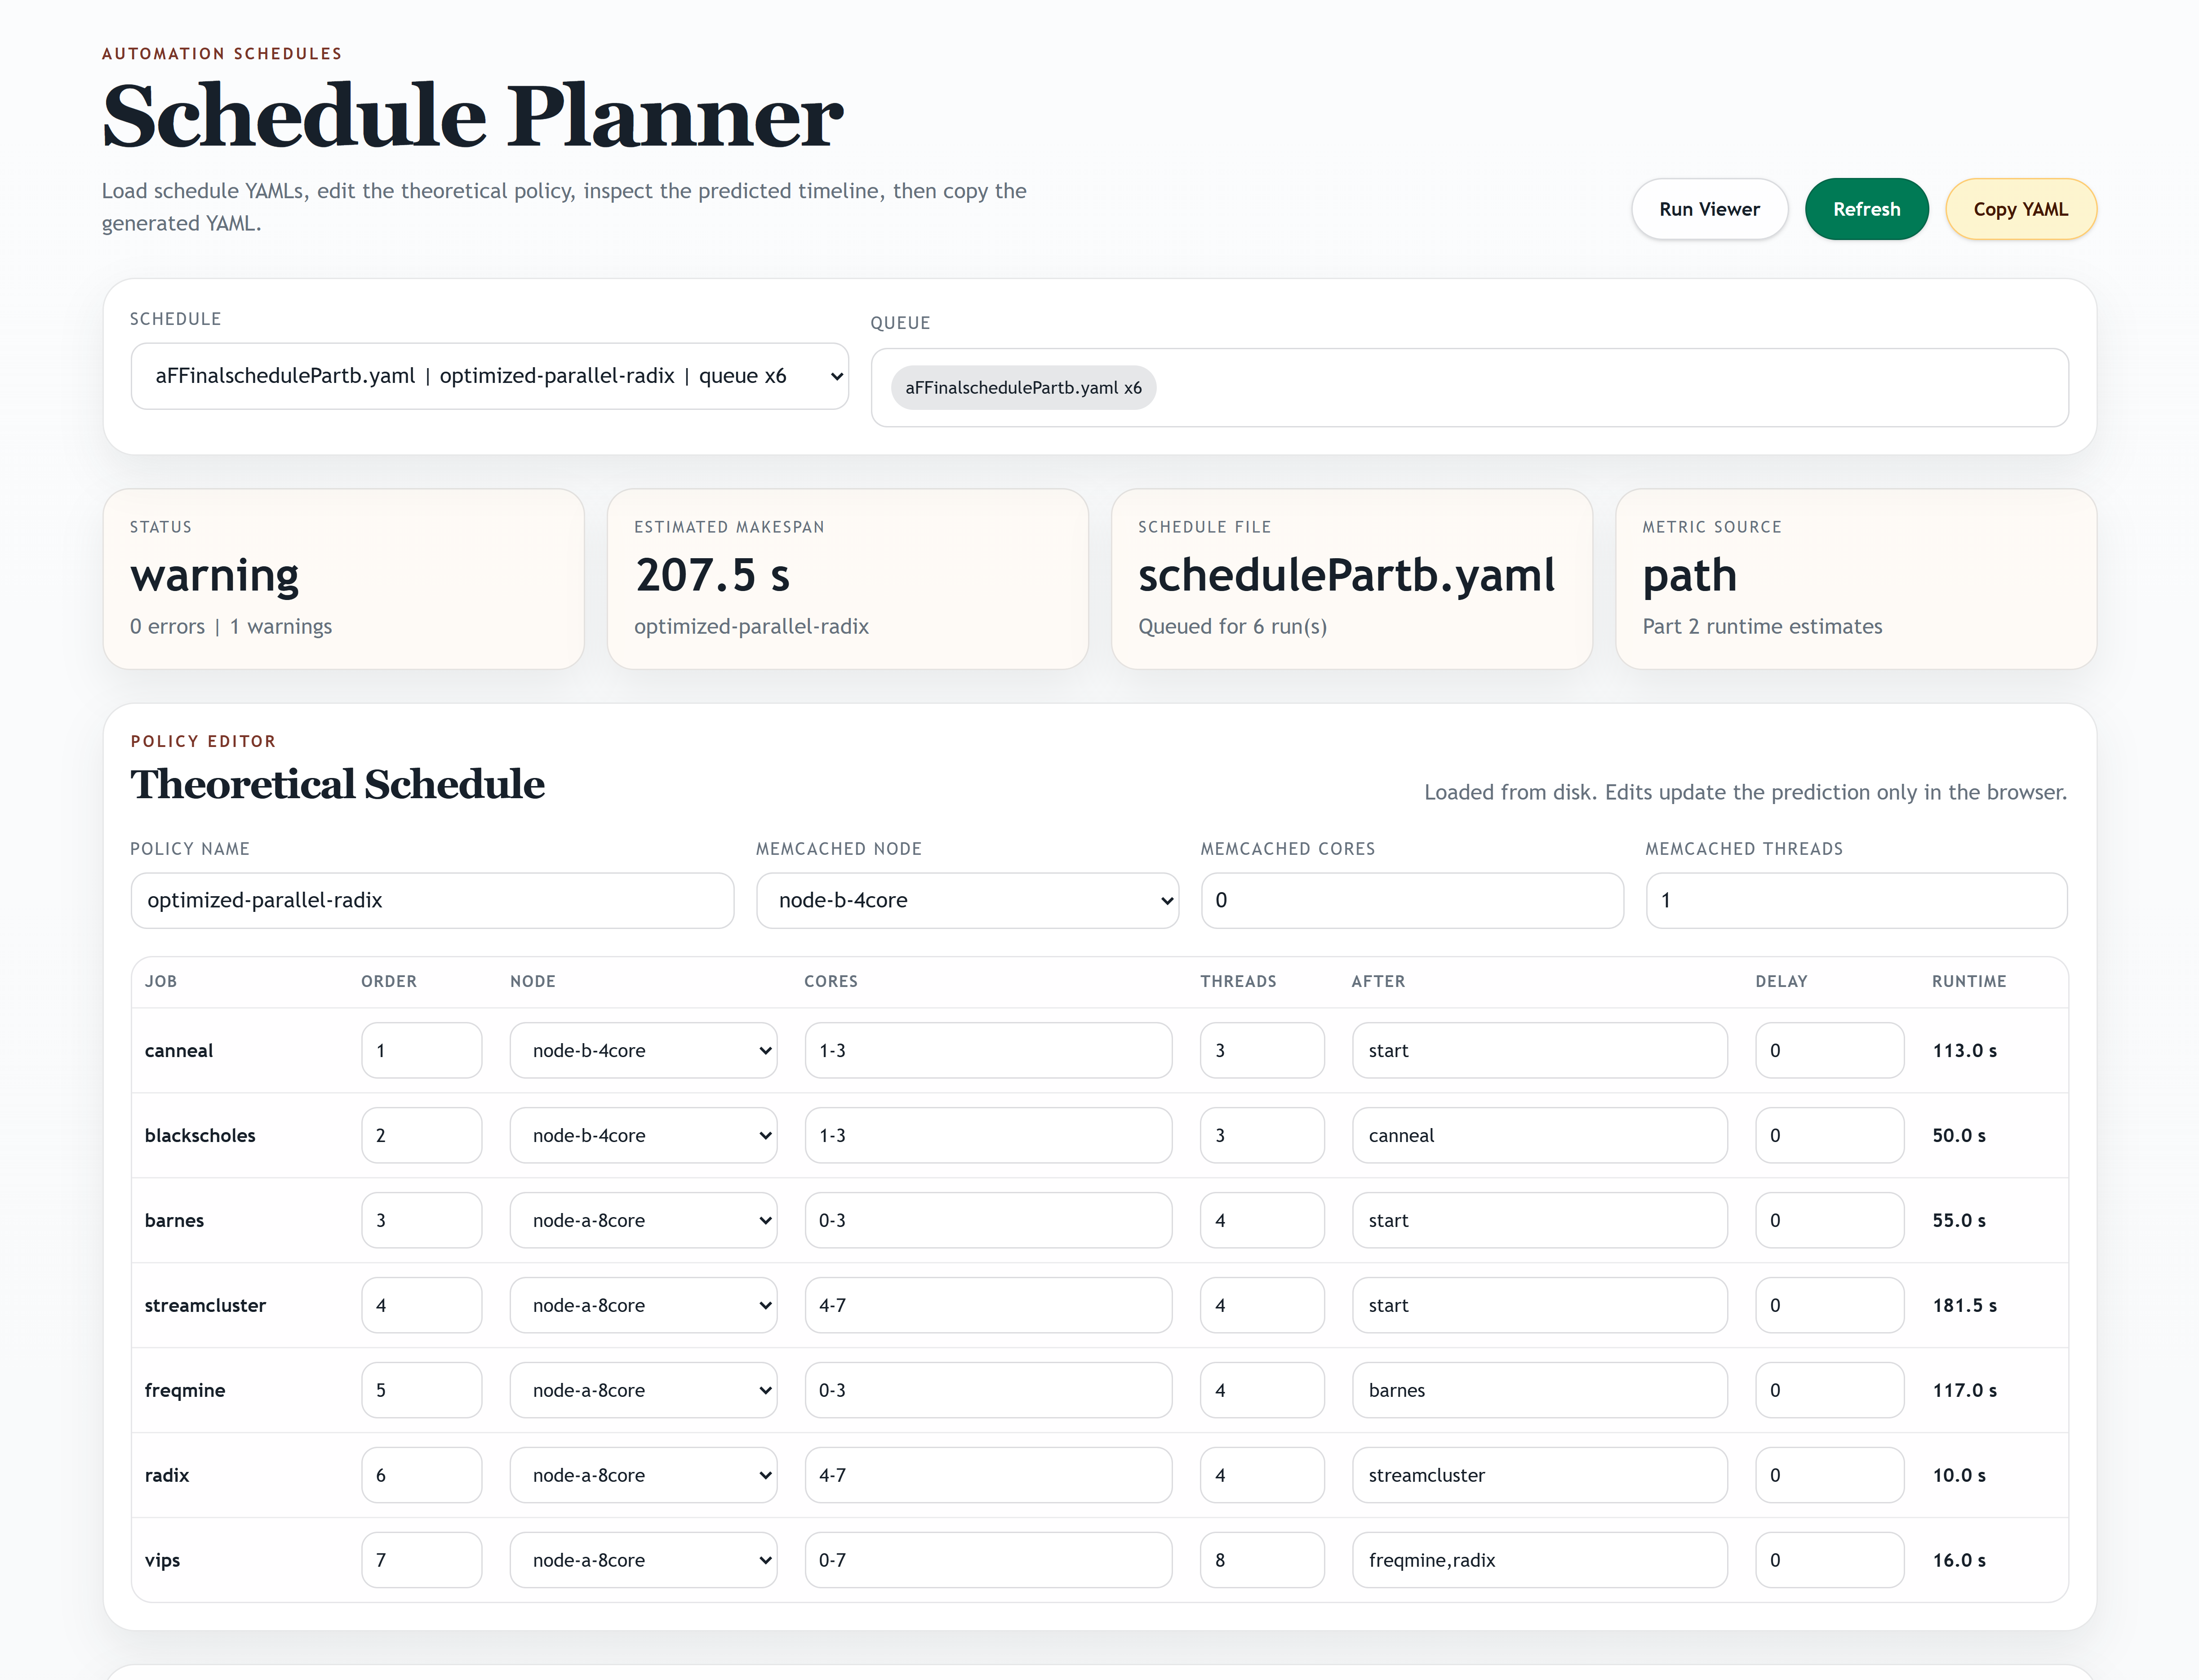
\includegraphics[width=\linewidth,height=0.40\textheight,keepaspectratio]{figures/part3/planner.png}
        \par\vspace{0.2em}
        {\small Schedule planner: YAML schedules, predicted makespan, warnings,
        and editable node/core/thread/dependency choices.\par}
    \end{minipage}

    \vspace{2em}

    \begin{minipage}{\linewidth}
        \centering
        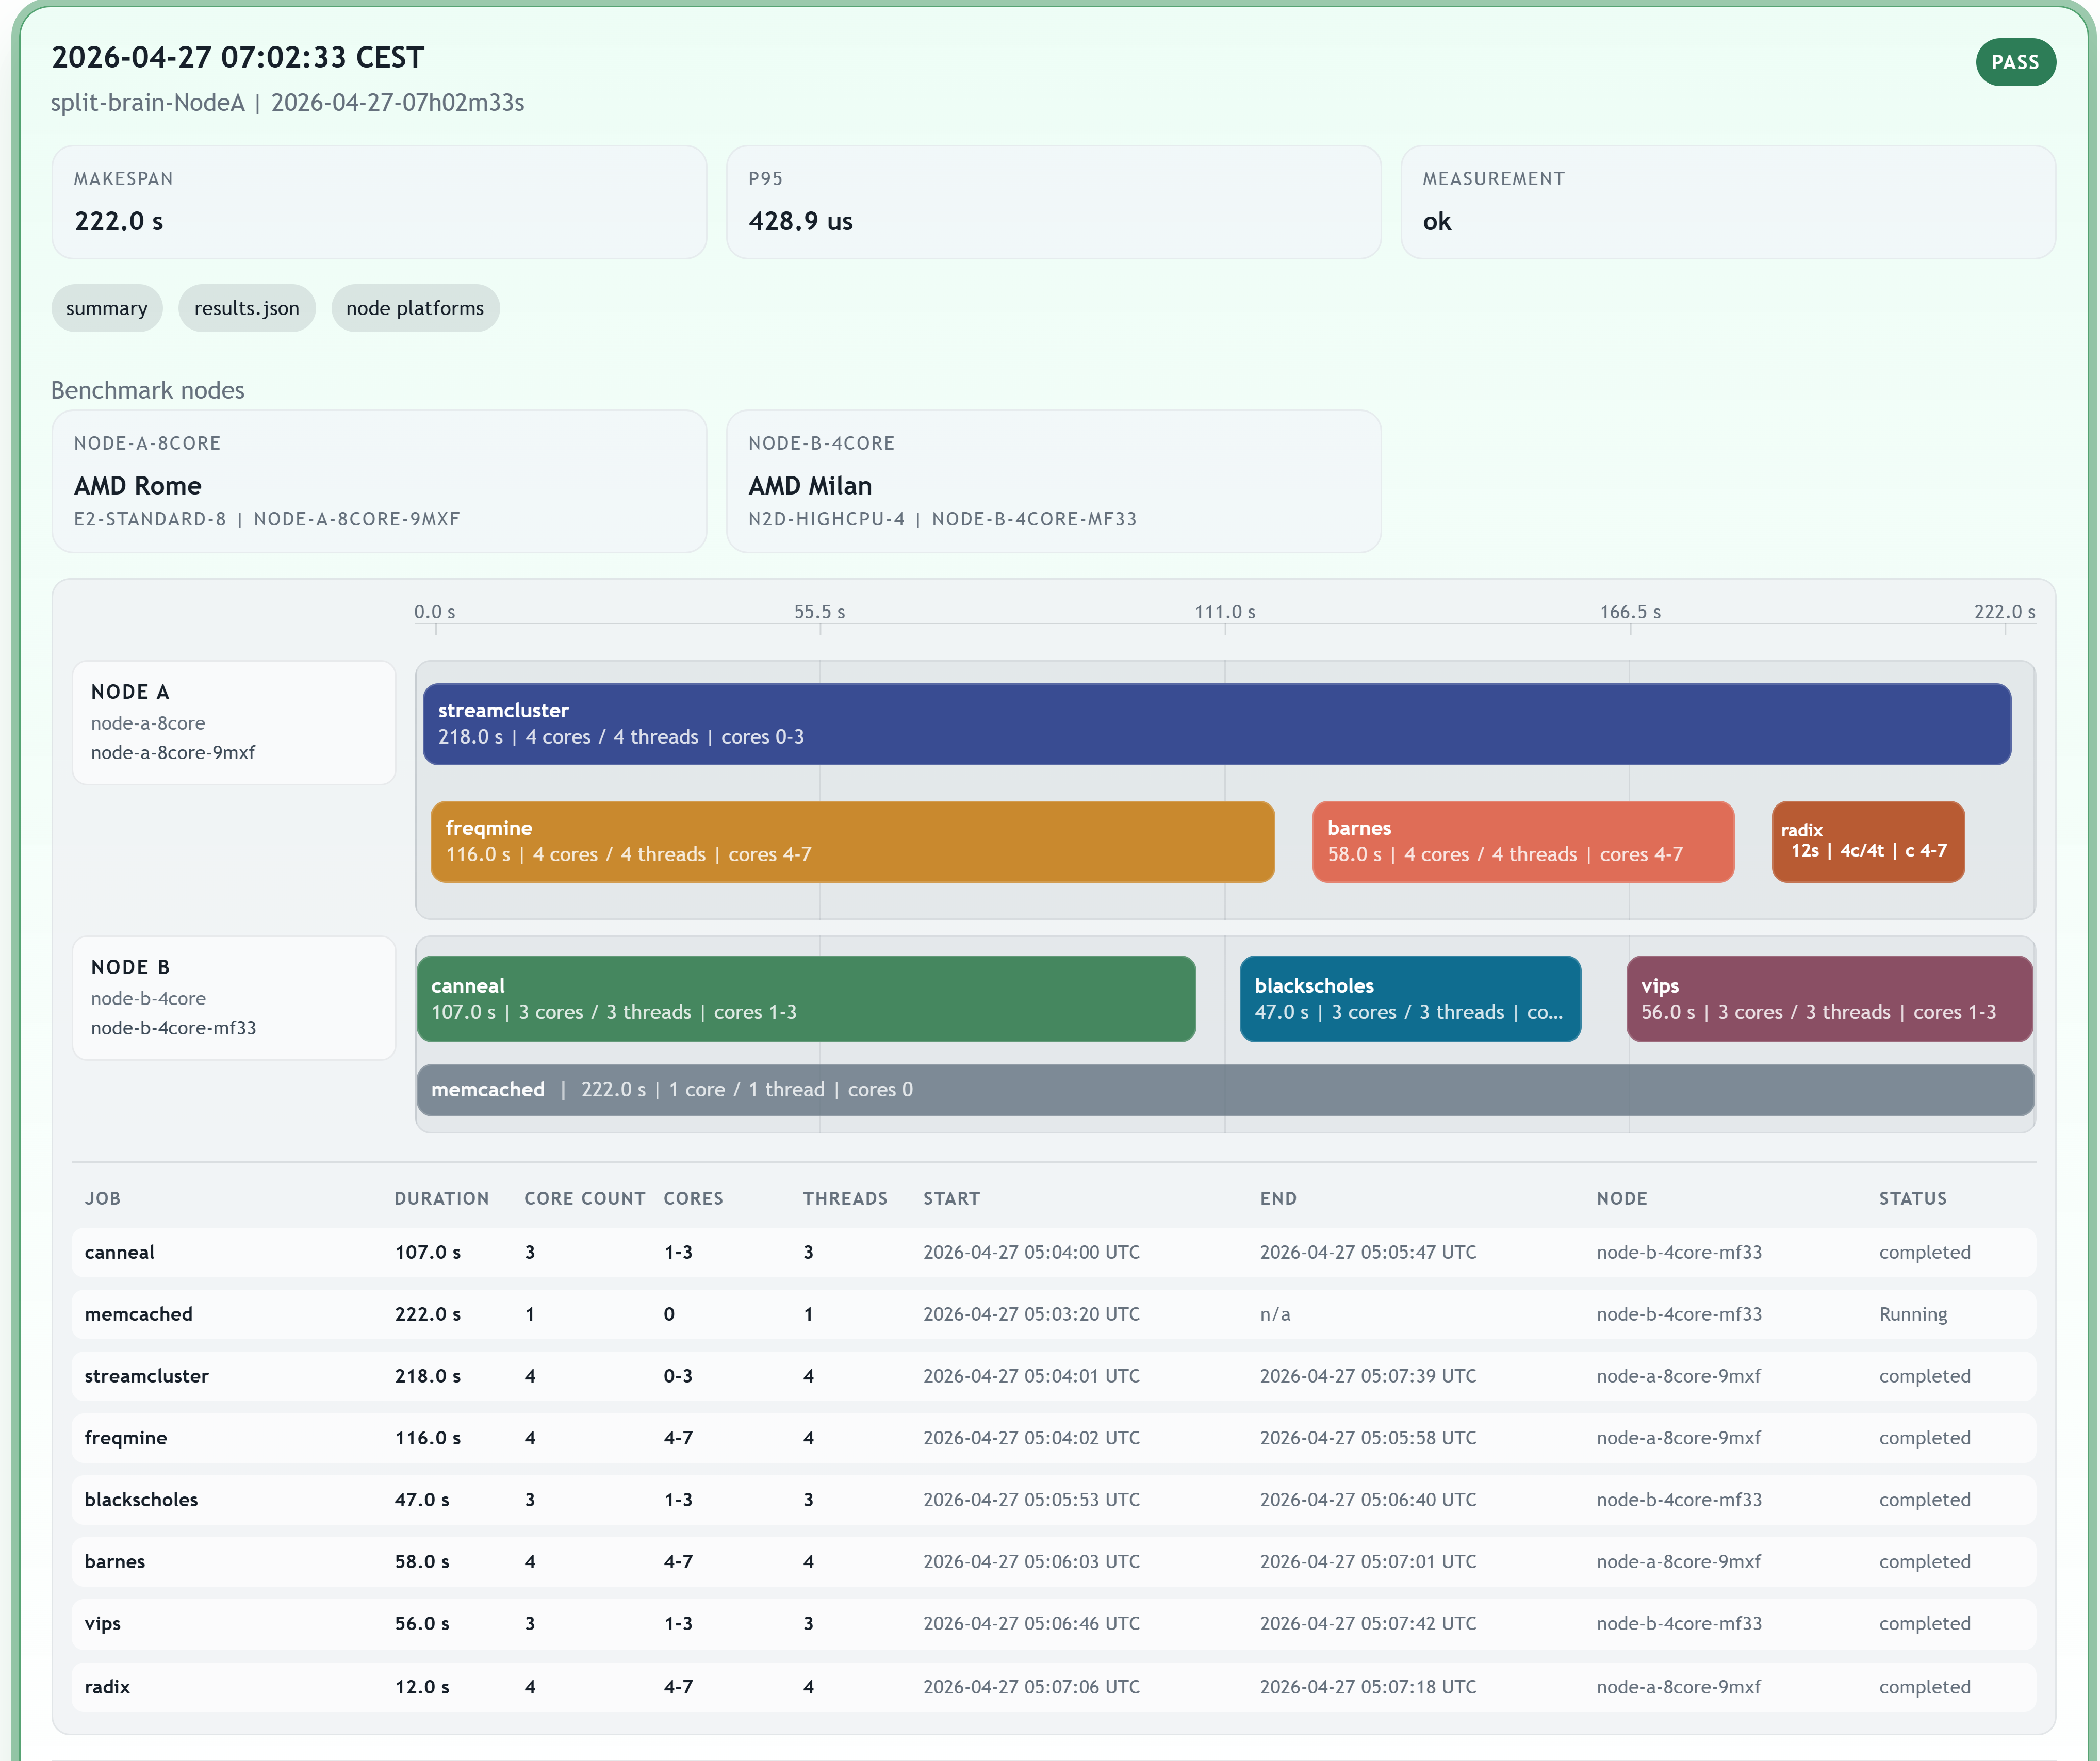
\includegraphics[width=\linewidth,height=0.40\textheight,keepaspectratio]{figures/part3/run.png}
        \par\vspace{0.2em}
        {\small Run viewer: measured makespan, detected node platforms, and the
        horizontal per-node job timeline.\par}
    \end{minipage}
\end{figure}

\clearpage
\section*{Appendix: Automation Script Structure}

\newcommand{\AutomationTreeFont}{\fontsize{11pt}{13pt}\selectfont}

\begin{Verbatim}[formatcom=\AutomationTreeFont,frame=single,framesep=2mm]
automation/
|-- cli.py                     # command-line entrypoint
|-- cluster.py                 # kOps/kubectl/gcloud wrappers
|   `-- node discovery, canonical labels, SSH helpers
|-- provision.py               # client bootstrap checks
|   `-- mcperf-agent readiness
|-- config.py                  # experiment/policy/queue YAML
|   `-- dependency and core/thread validation
|-- catalog.py                 # workload metadata
|-- cpu_sets.py                # CPU-set parsing and overlap checks
|-- manifests.py               # memcached, pre-cache Pod, Jobs
|-- runner.py                  # warmup, memcached, async DAG
|   `-- scheduler polling and artifact collection
|-- collect.py                 # pod logs and result collection
|-- metrics.py                 # SLO, latency, throughput, runtime
|-- timing.py                  # phase timing and makespan utilities
|-- results.py                 # summaries and best-run ranking
|-- audit.py                   # static audit and contention warnings
|-- runtime_stats.py           # run-derived runtime estimates
|-- viewer.py                  # local HTTP visualization server
|-- viewer_data.py             # run-viewer API and timeline model
|-- schedule_viewer_data.py    # planner API and prediction model
|-- gui.py                     # desktop schedule helper
|-- export.py                  # submission export helpers
|-- debug.py                   # diagnostics
|-- utils.py                   # shared utilities
|-- viewer_static/
|   |-- index.html             # run viewer page
|   |-- schedules.html         # schedule planner page
|   |-- app.js                 # run viewer frontend
|   |-- schedules.js           # schedule planner frontend
|   |-- timeline.js            # horizontal timeline rendering
|   `-- styles.css             # shared viewer styling
|-- schedules/                 # hand-crafted and candidate YAML policies
`-- runs/                      # policy snapshots, manifests, logs, results
\end{Verbatim}
